% Arquivo LaTeX de exemplo de dissertação/tese a ser apresentada à CPG do IME-USP
%
% Criação: Jesús P. Mena-Chalco
% Revisão: Fabio Kon e Paulo Feofiloff
% Adaptação para UTF8, biblatex e outras melhorias: Nelson Lago
%
% Except where otherwise indicated, these files are distributed under
% the MIT Licence. The example text, which includes the tutorial and
% examples as well as the explanatory comments in the source, are
% available under the Creative Commons Attribution International
% Licence, v4.0 (CC-BY 4.0) - https://creativecommons.org/licenses/by/4.0/


%%%%%%%%%%%%%%%%%%%%%%%%%%%%%%%%%%%%%%%%%%%%%%%%%%%%%%%%%%%%%%%%%%%%%%%%%%%%%%%%
%%%%%%%%%%%%%%%%%%%%%%%%%%%%%%% PREÂMBULO LaTeX %%%%%%%%%%%%%%%%%%%%%%%%%%%%%%%%
%%%%%%%%%%%%%%%%%%%%%%%%%%%%%%%%%%%%%%%%%%%%%%%%%%%%%%%%%%%%%%%%%%%%%%%%%%%%%%%%

% A opção twoside (frente-e-verso) significa que a aparência das páginas pares
% e ímpares pode ser diferente. Por exemplo, as margens podem ser diferentes ou
% os números de página podem aparecer à direita ou à esquerda alternadamente.
% Mas nada impede que você crie um documento "só frente" e, ao imprimir, faça
% a impressão frente-e-verso.
%
% Aqui também definimos a língua padrão do documento (a última da lista) e
% línguas adicionais. Para teses do IME, no mínimo português e inglês são
% obrigatórios, porque independentemente da língua principal do texto é
% preciso fornecer o resumo nessas duas línguas. LaTeX aceita alguns nomes
% diferentes para a língua portuguesa; dentre as opções, prefira sempre
% "brazilian" para português brasileiro e "portuguese" para português europeu.
%\documentclass[a4paper,12pt,twoside,brazilian,english]{book}
\documentclass[a4paper,12pt,twoside,english,brazilian]{book}

% O preâmbulo de um documento LaTeX pode ser razoavelmente longo. Neste
% modelo, optamos por reduzi-lo, colocando praticamente tudo do preâmbulo
% nas packages "imegoodies" e "imelooks".
%
% imegoodies carrega diversas packages muito úteis e populares (algumas
% são praticamente obrigatórias, como amsmath, babel, array etc.). É
% uma boa ideia usá-la com outros documentos também. Ela inclui vários
% comentários explicativos e dicas de uso; não tenha medo de alterá-la
% conforme a necessidade.
%
% imelooks carrega algumas packages e configurações que definem a
% aparência do documento; você também pode querer usá-la (ou partes
% dela) com outros documentos para obter as mesmas fontes, margens
% etc. Tal como "imegoodies", pode valer a pena ler os comentários
% e fazer modificações nessa package. Com a opção "thesis", imelooks
% também define os comandos para capa, folha de rosto etc.
\usepackage{imegoodies}
\usepackage[thesis]{imelooks}

%\nocolorlinks % para impressão em P&B

% Diretórios onde estão as figuras; com isso, não é necessário (mas
% é permitido) colocar o caminho completo em \includegraphics. Note
% que a extensão nunca é necessária (mas é permitida), ou seja, o
% resultado é o mesmo com "\includegraphics{figuras/foto.jpeg}",
% "\includegraphics{foto.jpeg}", "\includegraphics{figuras/foto}"
% ou "\includegraphics{foto}".
\graphicspath{{figuras/},{fig/},{logos/},{img/},{images/},{imagens/}}

% Comandos rápidos para mudar de língua:
% \en -> muda para o inglês
% \br -> muda para o português
% \texten{blah} -> o texto "blah" é em inglês
% \textbr{blah} -> o texto "blah" é em português
\babeltags{br = brazilian, en = english}


%%%%%%%%%%%%%%%%%%%%%%%%%%%%%%%%%%%%%%%%%%%%%%%%%%%%%%%%%%%%%%%%%%%%%%%%%%%%%%%%
%%%%%%%%%%%%%%%%%%%%%%%%%%%%%%%%%% METADADOS %%%%%%%%%%%%%%%%%%%%%%%%%%%%%%%%%%%
%%%%%%%%%%%%%%%%%%%%%%%%%%%%%%%%%%%%%%%%%%%%%%%%%%%%%%%%%%%%%%%%%%%%%%%%%%%%%%%%

% O arquivo com os dados bibliográficos para biblatex; você pode usar
% este comando mais de uma vez para acrescentar múltiplos arquivos
\addbibresource{bibliografia.bib}

% Este comando permite acrescentar itens à lista de referências sem incluir
% uma referência de fato no texto (pode ser usado em qualquer lugar do texto)
%\nocite{bronevetsky02,schmidt03:MSc, FSF:GNU-GPL, CORBA:spec, MenaChalco08}
% Com este comando, todos os itens do arquivo .bib são incluídos na lista
% de referências
%\nocite{*}

% É possível definir como determinadas palavras podem (ou não) ser
% hifenizadas; no entanto, a hifenização automática geralmente funciona bem
\babelhyphenation{documentclass latexmk soft-ware clsguide} % todas as línguas
\babelhyphenation[brazilian]{Fu-la-no}
\babelhyphenation[english]{what-ever}

% Estes comandos definem o título e autoria do trabalho e devem sempre ser
% definidos, pois além de serem utilizados para criar a capa, também são
% armazenados nos metadados do PDF. O subtítulo é opcional.
\title{Uma abordagem estocástica do Modelo de Lorenz 80}
\translatedtitle{A stochastic approach for the Lorenz 80 model}

\author{Lucas Amaral Taylor}

\def\profa{Prof\kern.02em.\kern-.07emª\kern.07em}
\def\dra{Dr\kern-.04em.\kern-.11emª\kern.07em}

% Para TCCs, este comando define o supervisor
\orientador{Prof. Dr. Breno Raphaldini Ferreira da Silva}


\banca{
  \profa{} \dra{} Fulana de Tal (orientadora) -- IME-USP [sem ponto final],
  % Em inglês, não há o "ª"
  %Prof. Dr. Fulana de Tal (advisor) -- IME-USP [sem ponto final],
  Prof. Dr. Ciclano de Tal -- IME-USP [sem ponto final],
  \profa{} \dra{} Convidada de Tal -- IMPA [sem ponto final],
}

% A página de rosto da versão para depósito (ou seja, a versão final
% antes da defesa) deve ser diferente da página de rosto da versão
% definitiva (ou seja, a versão final após a incorporação das sugestões
% da banca).
\tipotese{
  %mestrado,
  %doutorado,
  tcc,
  %definitiva, % É a versão para defesa ou a versão definitiva?
  %quali, % É qualificação?
  programa={Matemática Aplicada e Computacional},
}

\defesa{
  local={São Paulo},
  data=2017-08-10, % YYYY-MM-DD
}

% Se não houve bolsa, remova
%
% Norma sobre agradecimento por auxílios da FAPESP:
% https://fapesp.br/11789/referencia-ao-apoio-da-fapesp-em-todas-as-formas-de-divulgacao
%
% Norma sobre agradecimento por auxílios da CAPES (Portaria 206,
% de 4 de Setembro de 2018):
% https://www.in.gov.br/materia/-/asset_publisher/Kujrw0TZC2Mb/content/id/39729251/do1-2018-09-05-portaria-n-206-de-4-de-setembro-de-2018-39729135
%
%\apoio{O presente trabalho foi realizado com apoio da Coordenação
%      de Aperfeiçoamento\\ de Pessoal de Nível Superior -- Brasil
%      (CAPES) -- Código de Financiamento 001} % o código é sempre 001
%
%\apoio{This study was financed in part by the Coordenação de
%      Aperfeiçoamento\\ de Pessoal de Nível Superior -- Brasil
%      (CAPES) -- Finance Code 001} % o código é sempre 001
%
%\apoio{Durante o desenvolvimento deste trabalho, o autor recebeu\\
%      auxílio financeiro da FAPESP -- processo nº aaaa/nnnnn-d}
%
%\apoio{During the development if this work, the author received\\
%      financial support from FAPESP -- grant \#aaaa/nnnnn-d}
\apoio{}

% A licença do seu trabalho. Use CC-BY, CC-BY-NC, CC-BY-ND, CC-BY-SA,
% CC-BY-NC-SA ou CC-BY-NC-ND para escolher a licença Creative Commons
% correspondente (o sistema insere automaticamente o texto da licença).
% Se quiser estabelecer regras diferentes para o uso de seu trabalho,
% converse com seu orientador e coloque o texto da licença aqui, mas
% observe que apenas TCCs sob alguma licença Creative Commons serão
% acrescentados ao BDTA. Se você tem alguma intenção de publicar o
% trabalho comercialmente no futuro, sugerimos a licença CC-BY-NC-ND.
%
%\direitos{CC-BY-NC-ND}
%
%\direitos{Autorizo a reprodução e divulgação total ou parcial deste
%          trabalho, por qualquer meio convencional ou eletrônico,
%          para fins de estudo e pesquisa, desde que citada a fonte.}
%
%\direitos{I authorize the complete or partial reproduction and disclosure
%          of this work by any conventional or electronic means for study
%          and research purposes, provided that the source is acknowledged.}
%
\direitos{CC-BY}

% Para gerar a ficha catalográfica, acesse https://fc.ime.usp.br/,
% preencha o formulário e escolha a opção "Gerar Código LaTeX".
% Basta copiar e colar o resultado aqui.
\fichacatalografica{}


%%%%%%%%%%%%%%%%%%%%%%%%%%%%%%%%%%%%%%%%%%%%%%%%%%%%%%%%%%%%%%%%%%%%%%%%%%%%%%%%
%%%%%%%%%%%%%%%%%%%%%%% AQUI COMEÇA O CONTEÚDO DE FATO %%%%%%%%%%%%%%%%%%%%%%%%%
%%%%%%%%%%%%%%%%%%%%%%%%%%%%%%%%%%%%%%%%%%%%%%%%%%%%%%%%%%%%%%%%%%%%%%%%%%%%%%%%

\begin{document}

%%%%%%%%%%%%%%%%%%%%%%%%%%% CAPA E PÁGINAS INICIAIS %%%%%%%%%%%%%%%%%%%%%%%%%%%%

% Aqui começa o conteúdo inicial que aparece antes do capítulo 1, ou seja,
% página de rosto, resumo, sumário etc. O comando frontmatter faz números
% de página aparecem em algarismos romanos ao invés de arábicos e
% desabilita a contagem de capítulos.
\frontmatter

\pagestyle{plain}

\onehalfspacing % Espaçamento 1,5 na capa e páginas iniciais

\maketitle % capa e folha de rosto

%%%%%%%%%%%%%%%% DEDICATÓRIA, AGRADECIMENTOS, RESUMO/ABSTRACT %%%%%%%%%%%%%%%%%%

\begin{dedicatoria}
Na verdade, na verdade vos digo que, se o grão de trigo, caindo na terra, não morrer, fica ele só; mas se morrer, dá muito fruto. 

João 12:24
\end{dedicatoria}

% Reinicia o contador de páginas (a próxima página recebe o número "i") para
% que a página da dedicatória não seja contada.
\pagenumbering{roman}

% Agradecimentos:
% Se o candidato não quer fazer agradecimentos, deve simplesmente eliminar
% esta página. A epígrafe, obviamente, é opcional; é possível colocar
% epígrafes em todos os capítulos. O comando "\chapter*" faz esta seção
% não ser incluída no sumário.
\chapter*{Agradecimentos}
\epigrafe{Do. Or do not. There is no try.}{Mestre Yoda}

Texto texto texto texto texto texto texto texto texto texto texto texto texto
texto texto texto texto texto texto texto texto texto texto texto texto texto
texto texto texto texto texto texto texto texto texto texto texto texto texto
texto texto texto texto. Texto opcional.

%!TeX root=../tese.tex
%("dica" para o editor de texto: este arquivo é parte de um documento maior)
% para saber mais: https://tex.stackexchange.com/q/78101

% As palavras-chave são obrigatórias, em português e em inglês, e devem ser
% definidas antes do resumo/abstract. Acrescente quantas forem necessárias.
\palavraschave{Palavra-chave1, Palavra-chave2, Palavra-chave3}

\keywords{Keyword1,Keyword2,Keyword3}

% O resumo é obrigatório, em português e inglês. Estes comandos também
% geram automaticamente a referência para o próprio documento, conforme
% as normas sugeridas da USP.
\resumo{
Elemento obrigatório, constituído de uma sequência de frases concisas e
objetivas, em forma de texto. Deve apresentar os objetivos, métodos empregados,
resultados e conclusões. O resumo deve ser redigido em parágrafo único, conter
no máximo 500 palavras e ser seguido dos termos representativos do conteúdo do
trabalho (palavras-chave). Deve ser precedido da referência do documento.
Texto texto texto texto texto texto texto texto texto texto texto texto texto
texto texto texto texto texto texto texto texto texto texto texto texto texto
texto texto texto texto texto texto texto texto texto texto texto texto texto
texto texto texto texto texto texto texto texto texto texto texto texto texto
texto texto texto texto texto texto texto texto texto texto texto texto texto
texto texto texto texto texto texto texto texto.
Texto texto texto texto texto texto texto texto texto texto texto texto texto
texto texto texto texto texto texto texto texto texto texto texto texto texto
texto texto texto texto texto texto texto texto texto texto texto texto texto
texto texto texto texto texto texto texto texto texto texto texto texto texto
texto texto.
}

\abstract{
Elemento obrigatório, elaborado com as mesmas características do resumo em
língua portuguesa. De acordo com o Regimento da Pós-Graduação da USP (Artigo
99), deve ser redigido em inglês para fins de divulgação. É uma boa ideia usar
o sítio \url{www.grammarly.com} na preparação de textos em inglês.
Text text text text text text text text text text text text text text text text
text text text text text text text text text text text text text text text text
text text text text text text text text text text text text text text text text
text text text text text text text text text text text text.
Text text text text text text text text text text text text text text text text
text text text text text text text text text text text text text text text text
text text text.
}



%%%%%%%%%%%%%%%%%%%%%%%%%%% LISTAS DE FIGURAS ETC. %%%%%%%%%%%%%%%%%%%%%%%%%%%%%

% Como as listas que se seguem podem não incluir uma quebra de página
% obrigatória, inserimos uma quebra manualmente aqui.
\cleardoublepage

% Todas as listas são opcionais; Usando "\chapter*" elas não são incluídas
% no sumário. As listas geradas automaticamente também não são incluídas por
% conta das opções "notlot" e "notlof" que usamos para a package tocbibind.

% Normalmente, "\chapter*" faz o novo capítulo iniciar em uma nova página, e as
% listas geradas automaticamente também por padrão ficam em páginas separadas.
% Como cada uma destas listas é muito curta, não faz muito sentido fazer isso
% aqui, então usamos este comando para desabilitar essas quebras de página.
% Se você preferir, comente as linhas com esse comando e des-comente as linhas
% sem ele para criar as listas em páginas separadas. Observe que você também
% pode inserir quebras de página manualmente (com \clearpage, veja o exemplo
% mais abaixo).
\newcommand\disablenewpage[1]{{\let\clearpage\par\let\cleardoublepage\par #1}}

% Nestas listas, é melhor usar "raggedbottom" (veja basics.tex). Colocamos
% a opção correspondente e as listas dentro de um grupo para ativar
% raggedbottom apenas temporariamente.
\bgroup
\raggedbottom

% Quebra de página manual
\clearpage

%%%%% Listas criadas automaticamente

% Você pode escolher se quer ou não permitir a quebra de página
%\listoffigures
\disablenewpage{\listoffigures}

% Você pode escolher se quer ou não permitir a quebra de página
%\listoftables
\disablenewpage{\listoftables}

% Esta lista é criada "automaticamente" pela package float quando
% definimos o novo tipo de float "program" (em utils.tex)
% Você pode escolher se quer ou não permitir a quebra de página
%\listof{program}{\programlistname}
\disablenewpage{\listof{program}{\programlistname}}

% Sumário (obrigatório)
\tableofcontents

\egroup % Final de "raggedbottom"

% Referências indiretas ("x", veja "y") para o índice remissivo (opcionais,
% pois o índice é opcional). É comum colocar esses itens no final do documento,
% junto com o comando \printindex, mas em alguns casos isso torna necessário
% executar texindy (ou makeindex) mais de uma vez, então colocar aqui é melhor.
\index{Inglês|see{Língua estrangeira}}
\index{Figuras|see{Floats}}
\index{Tabelas|see{Floats}}
\index{Código-fonte|see{Floats}}
\index{Subcaptions|see{Subfiguras}}
\index{Sublegendas|see{Subfiguras}}
\index{Equações|see{Modo matemático}}
\index{Fórmulas|see{Modo matemático}}
\index{Rodapé, notas|see{Notas de rodapé}}
\index{Captions|see{Legendas}}
\index{Versão original|see{Tese/Dissertação, versões}}
\index{Versão corrigida|see{Tese/Dissertação, versões}}
\index{Palavras estrangeiras|see{Língua estrangeira}}
\index{Floats!Algoritmo|see{Floats, ordem}}


%%%%%%%%%%%%%%%%%%%%%%%%%%%%%%%% CAPÍTULOS %%%%%%%%%%%%%%%%%%%%%%%%%%%%%%%%%%%%%

% Aqui vai o conteúdo principal do trabalho, ou seja, os capítulos que compõem
% a dissertação/tese. O comando mainmatter reinicia a contagem de páginas,
% modifica a numeração para números arábicos e ativa a contagem de capítulos.
\mainmatter

\pagestyle{mainmatter}

% Espaçamento simples
\singlespacing

% A introdução não tem número de capítulo, então os cabeçalhos também não
\pagestyle{unnumberedchapter}
%!TeX root=../tese.tex
%("dica" para o editor de texto: este arquivo é parte de um documento maior)
% para saber mais: https://tex.stackexchange.com/q/78101

%% ------------------------------------------------------------------------- %%

% "\chapter" cria um capítulo com número e o coloca no sumário; "\chapter*"
% cria um capítulo sem número e não o coloca no sumário. A introdução não
% deve ser numerada, mas deve aparecer no sumário. Por conta disso, este
% modelo define o comando "\chapter**".
\chapter**{Introdução}
\label{cap:introducao}

\enlargethispage{.5\baselineskip}

Escrever bem é uma arte que exige muita técnica e dedicação e,
consequentemente, há vários bons livros sobre como escrever uma boa
dissertação ou tese. Um dos trabalhos pioneiros e mais conhecidos nesse
sentido é o livro de Umberto~\citet{eco:09} intitulado \emph{Como se faz
uma tese}; é uma leitura bem interessante mas, como foi escrito em 1977 e
é voltado para trabalhos de graduação na Itália, não se aplica tanto a nós.

Sobre a escrita acadêmica em geral, John Carlis disponibilizou um texto curto
e interessante~\citep{carlis:09} em que advoga a preparação de um único
rascunho da tese antes da versão final. Mais importante que isso, no
entanto, são os vários \textit{insights} dele sobre a escrita acadêmica.
Dois outros bons livros sobre o tema são \emph{The Craft of Research}~\citep{craftresearch}
e \emph{The Dissertation Journey}~\citep{dissertjourney}. Além disso,
a USP tem uma compilação de normas relativas à produção de documentos
acadêmicos~\citep{usp:guidelines} que pode ser utilizada como referência.

Para a escrita de textos especificamente sobre Ciência da Computação, o
livro de Justin Zobel, \emph{Writing for Computer Science}~\citep{zobel:04}
é uma leitura obrigatória. O livro \emph{Metodologia de Pesquisa para
Ciência da Computação} de Raul Sidnei~\citet{waz:09}
também merece uma boa lida. Já para a área de Matemática, dois livros
recomendados são o de Nicholas Higham, \emph{Handbook of Writing for
Mathematical Sciences}~\citep{Higham:98} e o do criador do \TeX{}, Donald
Knuth, juntamente com Tracy Larrabee e Paul Roberts, \emph{Mathematical
Writing}~\citep{Knuth:96}.

Apresentar os resultados de forma simples, clara e completa é uma tarefa que
requer inspiração. Nesse sentido, o livro de Edward~\citet{tufte01:visualDisplay},
\emph{The Visual Display of Quantitative Information}, serve de ajuda na
criação de figuras que permitam entender e interpretar dados/resultados de forma
eficiente.

Além desse material, também vale muito a pena a leitura do trabalho de
Uri \citet{alon09:how}, no qual apresenta-se uma reflexão sobre a utilização
da Lei de Pareto para tentar definir/escolher problemas para as diferentes
fases da vida acadêmica. A direção dos novos passos para a continuidade da
vida acadêmica deveria ser discutida com seu orientador.

\section**{Considerações de estilo}
\label{sec:consideracoes_preliminares}

Normalmente, as citações não devem fazer parte da estrutura sintática da
frase\footnote{E não se deve abusar das notas de rodapé.\index{Notas de rodapé}}.
No entanto, usando referências em algum estilo autor-data (como o estilo
plainnat do \LaTeX{}), é comum que o nome do autor faça parte da frase. Nesses
casos, pode valer a pena mudar o formato da citação para não repetir o nome do
autor; no \LaTeX{}, isso pode ser feito usando os comandos
\textsf{\textbackslash{}citet}, \textsf{\textbackslash{}citep},
\textsf{\textbackslash{}citeyear} etc. documentados no pacote
natbib \citep{natbib}\index{natbib} (esses comandos são compatíveis com biblatex
usando a opção \textsf{natbib=true}, ativada por padrão neste modelo). Em geral,
portanto, as citações devem seguir estes exemplos:

\bgroup
\footnotesize
\begin{verbatim}
Modos de citação:
indesejável: [AF83] introduziu o algoritmo ótimo.
indesejável: (Andrew e Foster, 1983) introduziram o algoritmo ótimo.
certo: Andrew e Foster introduziram o algoritmo ótimo [AF83].
certo: Andrew e Foster introduziram o algoritmo ótimo (Andrew e Foster, 1983).
certo (\citet ou \citeyear): Andrew e Foster (1983) introduziram o algoritmo ótimo.
\end{verbatim}
\egroup

\enlargethispage{.5\baselineskip}

O uso desnecessário de termos em língua estrangeira deve ser evitado. No entanto,
quando isso for necessário, os termos devem aparecer \textit{em itálico}.
\index{Língua estrangeira}
% index permite acrescentar um item no indice remissivo

Uma prática recomendável na escrita de textos é descrever as
legendas\index{Legendas} das figuras e tabelas em forma auto-contida: as
legendas devem ser razoavelmente completas, de modo que o leitor possa entender
a figura sem ler o texto em que a figura ou tabela é citada.\index{Floats}

\section**{Ferramentas bibliográficas}

Embora seja possível pesquisar por material acadêmico na Internet usando
sistemas de busca ``comuns'', existem ferramentas dedicadas, como o
\textsf{Google Scholar}\index{Google Scholar} (\url{scholar.google.com}).
O \textsf{Web of Science}\index{Web of Science} (\url{webofscience.com})
e o \textsf{Scopus}\index{Scopus} (\url{scopus.com}) oferecem recursos
sofisticados e limitam a busca a periódicos com boa reputação acadêmica.
Essas duas plataformas não são gratuitas, mas os alunos da USP têm
acesso a elas através da instituição. Algumas editoras, como a ACM
(\url{dl.acm.org}) e a IEEE (\url{ieeexplore.ieee.org}), também têm
sistemas de busca bibliográfica. Todas essas ferramentas são capazes de
exportar os dados para o formato .bib, usado pelo \LaTeX{} (no Google
Scholar, é preciso ativar a opção correspondente nas preferências).
O sítio \url{liinwww.ira.uka.de/bibliography} também permite buscar e
baixar referências bibliográficas relevantes para a área de computação.

Lamentavelmente, ainda não existe um mecanismo de verificação ou validação
das informações nessas plataformas. Portanto, é fortemente sugerido validar
todas as informações de tal forma que as entradas bib estejam corretas.
De qualquer modo, tome muito cuidado na padronização das referências
bibliográficas: ou considere TODOS os nomes dos autores por extenso, ou TODOS
os nomes dos autores abreviados. Evite misturas inapropriadas.\looseness=-1

Apenas uma parte dos artigos acadêmicos de interesse está disponível livremente
na Internet; os demais são restritos a assinantes. A CAPES assina um grande
volume de publicações e disponibiliza o acesso a elas para diversas
universidades brasileiras, entre elas a USP, através do seu portal de
periódicos (\url{periodicos.capes.gov.br}). Existe uma extensão para os
navegadores Chrome e Firefox (\url{www.infis.ufu.br/capes-periodicos})
que facilita o uso cotidiano do portal.

Para manter um banco de dados organizado sobre artigos e outras fontes
bibliográficas relevantes para sua pesquisa, é altamente recomendável
que você use uma ferramenta como Zotero~(\url{zotero.org})\index{Zotero}
ou Mendeley~(\url{mendeley.com})\index{Mendeley}. Ambas podem exportar
seus dados no formato .bib, compatível com \LaTeX{}.

\pagestyle{mainmatter}
\chapter{O modelo de Lorenz 80 determinístico} \label{cap:ch01_lorenz_deterministico}

\section{Introdução} \label{sec:ch01_introducao}
Este capítulo tem como objetivo apresentar o modelo determinístico Lorenz 80. Para isso, começamos, na seção \ref{sec:ch01_geofisica}, com uma introdução aos conceitos básicos de geofísica, a fim de familiarizar o leitor com os fundamentos dessa área. Em seguida, na seção \ref{sec:ch01_apresentacao_do_modelo}, contextualizamos o modelo, discutindo os trabalhos que o precederam e as motivações por trás de sua formulação.

Na seção \ref{sec:ch01_agua_rasa}, introduzimos o modelo de água rasa, que serve de base para o desenvolvimento do Lorenz 80. A construção deste é detalhada na seção \ref{sec:ch01_construcao_do_modelo}. Por fim, a seção \ref{sec:ch01_simulacoes_deterministico} traz simulações computacionais realizadas com o modelo, acompanhadas de uma análise gráfica dos resultados.

\section{Breves considerações sobre geofísica} \label{sec:ch01_geofisica}

Nesta seção, reunimos um breve glossário com os principais conceitos de geofísica que servem de base para a compreensão do modelo de Lorenz 80. Todas as definições expostas abaixo estão detalhadas em \citet{Vallis2017}.
\begin{itemize}
    \item \textbf{Convecção.} Convecção é um processo de transferência de calor que ocorre em
    fluidos, como líquidos e gases. Esse fenômeno envolve o movimento do próprio
    fluido e a transferência energia térmica de uma região para outra.
	\item \textbf{Parâmetro de Coriolis.} A \textit{força de Coriolis} é uma quasi-força (ou pseudo-força) que surge devido à rotação da Terra. Quando analisamos o movimento de um corpo em um referencial rotativo, esse corpo parece sofrer a ação de uma força que desvia sua trajetória. Esse desvio é quantificado pelo parâmetro de Coriolis, definido pela expressão:
	      \begin{equation*}
	      	f = 2 \Omega \sin(\theta)
	      \end{equation*}
	      onde $\Omega$ representa a velocidade angular de rotação da Terra e $\theta$ é a latitude, ou seja, o ângulo entre a posição do ponto e o equador terrestre.
	      
	\item \textbf{Número de Rossby.} O número de Rossby é a razão entre a magnitude da aceleração relativa e a aceleração de Coriolis. É aproximado por:
	      \begin{equation*}
	      	Ro \equiv \frac{U}{fL},
	      \end{equation*}
	      
	      onde $U$ é a magnitude aproximada da velocidade horizontal e $L$ é uma escala de comprimento e $f$ é o parâmetro de Coriolis.
	      
	\item \textbf{Equilíbrio hidrostático.} Matematicamente, a equação do equilíbrio hidrostático é dada por:
	      \begin{equation}
	      	\frac{\partial p}{\partial z} = - \rho_0g, \label{eq:equilibrio_hidrostatico}
	      \end{equation}
	          
	      onde: $p$ é a pressão do fluido, $z$ é a coordenada vertical, $\rho_0$ é a densidade constante do fluido e $g$ é a aceleração da gravidade.
	\item \textbf{Conservação de massa.} Em um escoamento de fluido, a densidade pode variar de acordo com o tempo ou a posição. No entanto, a \textit{quantidade total de massa} do fluido permanece constante. Esse princípio estabelece que a massa não pode ser criada nem perdida durante o movimento.
	      
	\item \textbf{Equações quasi-geostróficas.} As equações quasi-geostróficas são equações  amplamente usadas em estudos teóricos da atmosfera e oceano. Elas atendem as seguintes características:
	      \begin{enumerate}
	      	\item O número de Rossby é pequeno;
	      	\item A escala do movimento não é significativamente maior do que a escala de deformação;
	      	\item As variações no parâmetro de Coriolis são pequenas;
	      	\item As escalas de tempo são advectivas, ou seja, $T=L/U$.
	      \end{enumerate}
\end{itemize}



\section{Motivação e apresentação do modelo} \label{sec:ch01_apresentacao_do_modelo}

Edward Norton Lorenz (1917-2008) foi um importante matemático e meteorologista responsável pela publicação de vários artigos com desenvolvimento de modelos na área de meteorologia e geofísica.

O mais famoso deles foi o artigo \textit{``Deterministic Nonperiodic Flow''}, publicado em 1963 \citet{Lorenz1963}. Nele, Lorenz desenvolveu um modelo matemático simplificado para a convecção atmosférica, composto por três equações diferenciais ordinárias, expressas abaixo:
\begin{align}
    \begin{cases}
        \frac{dx}{dt} & = \sigma(y-x)     \\
        \frac{dy}{dt} & = x(\rho - z) - y \\
        \frac{dz}{dt} & = xy - \beta z
    \end{cases},
    \label{eq:ch01-lorenz63}
\end{align}

onde $\sigma$ é o \textit{número de Prandtl}, que regula a sensibilidade entre $x$ e $y$; $\rho$ é o \textit{número de Rayleigh}, associado à magnitude da convecção; e $\beta$ está ligado à geometria da célula de convecção, influenciando a relação entre as taxas de $x$ e $z$.
    
O modelo acima, conhecido como Lorenz 63, é um sistema determinístico desenvolvido para representar sistemas hidrodinâmicos ideais e dissipativos de força. O Lorenz 63 tornou-se amplamente conhecido por sua alta sensibilidade às condições iniciais — pequenas alterações nas variáveis $x_0$, $y_0$ e $z_0$ podem levar a trajetórias completamente distintas no espaço de fases. Essa sensibilidade extrema é uma característica caótica do modelo.

Em 1980, Lorenz publica o artigo intitulado ``\textit{Attractor Sets and Quasi-Geostrophic Equilibrium }'' \citep{Lorenz1980}. Neste artigo, Lorenz apresenta a construção e a simulação de dois modelos distintos: o primeiro, é formado a partir das equações primitivas (PE) com nove EDOs (equações diferenciais ordinárias), derivado das equações de águas rasas com topografia e forçamento, enquanto o segundo é um modelo quasi-geostrófico (QG) com 3 EDOs, obtido ao descartar as variáveis associadas ao escoamento divergente $x$ e seus termos correspondentes. O modelo PE contém tanto ondas gravitacionais rápidas quanto oscilações quasi-geostróficas lentas, enquanto o modelo QG mantém apenas estas últimas, em um quadro simplificado para atmosfera de latitudes médias.


\section{O modelo de água-rasa} \label{sec:ch01_agua_rasa}
O modelo de água rasa descreve um fluido de densidade constante, em equilíbrio hidrostático, que pode ou não estar em rotação. Nele, a escala horizontal é significativamente maior que a profundidade. Esse fluido possui superfície livre e é limitado pelas bordas \citep{Vallis2017}. No caso considerado, adotamos a versão de uma única camada.

Para a construção do modelo de água-rasa, consideramos a equação do equilíbrio hidrostático, expressa em \eqref{eq:equilibrio_hidrostatico}. A partir das manipulações envolvendo os conceitos de momento e conservação de massa, detalhado em \citet{Vallis2017}, obtemos as equações que descrevem o modelo: 
\begin{align}
	\frac{\partial V}{\partial t} + (V \cdot \nabla)V + f \mathbf{k} \times V & = -g \nabla \eta \label{eq:agua-rasa-1} \\
	\frac{\partial \eta}{\partial t} + \nabla \cdot (\eta V)                  & = 0 \label{eq:agua-rasa-2}              
\end{align}

Onde:
\begin{itemize}
	\item $t$: tempo;
	\item $\mathbf{r}$: vetor de posição inicial;
	\item $V(t)$: Velocidade horizontal;
	\item $\eta(t)$: altura da superfície;
	\item $\mathbf{k}$: vetor da vertical.
\end{itemize}

\section{Construção dos modelos} \label{sec:ch01_construcao_do_modelo}
Nesta seção, apresentaremos a construção dos modelos apresentados no artigo \citet{Lorenz1980}. Como dito anteriormente, o modelo é construído a partir das equações de água-rasa com algumas particularidades descritas a seguir. 

Consideremos um fluido homogêneo e incompressível, ou seja, com densidade constante em todo o volume e volume invariável mesmo sob variações de pressão. O escoamento é predominantemente horizontal, descrito por uma velocidade $V(t, \mathbf{r})$ independente da altura, onde $\mathbf{r}$ representa o vetor de posição inicial.

A componente vertical da velocidade é determinada pela continuidade de massa. A superfície livre do fluido está localizada na altura $H + z(t, \mathbf{r})$, onde $H$ representa a profundidade média e a base se apoia sobre uma topografia variável $h(\mathbf{r})$. Temos também que $h(\mathbf{r})$ e $z(t, \mathbf{r})$ possuem média zero.

O sistema está sujeito à rotação planetária, com um parâmetro de Coriolis constante $f$. 
Tanto o campo de velocidades $V$ quanto a elevação da superfície $z$ sofrem dissipação difusiva, 
associada a movimentos de pequena escala: o termo $\nu$ representa o coeficiente de difusão viscosa (dissipação de momento) e $\kappa$ representa o coeficiente de difusão térmica. O modelo também inclui um termo de forçamento externo $F(\mathbf{r})$ e, por fim, adota-se a hipótese de equilíbrio hidrostático.


A partir da descrição acima, podemos construir o seguinte diagrama:
\begin{figure}[H]
	\centering
	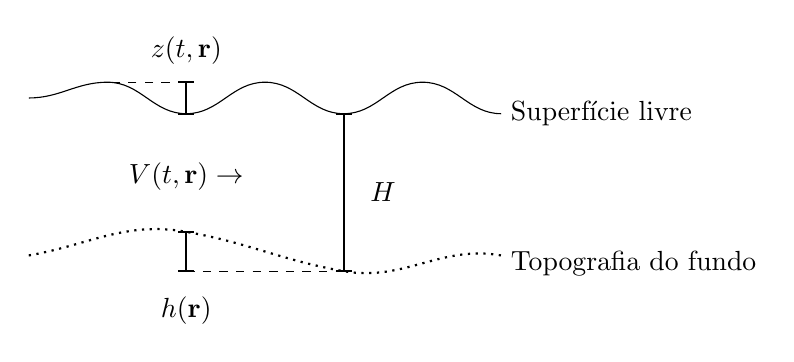
\begin{tikzpicture}[scale=1] 
						
		% Superfície livre
		\draw[above] (0,4) to[out=0,in=180] (1,4.2) 
		to[out=0,in=180] (2,3.8)
		to[out=0,in=180] (3,4.2)
		to[out=0,in=180] (4,3.8)
		to[out=0,in=180] (5,4.2)
		to[out=0,in=180] (6,3.8);
		\node[right] at (6,3.8) {Superfície livre};
						
		% Linha tracejada de referência para z
		\draw[dashed] (2,4.2) -- (1,4.2);
						
		% Desvio da superfície z
		\draw[thick] (2,3.8) -- (2,4.2);
		\draw[thick] (1.9,3.8) -- (2.1,3.8); % traço inferior
		\draw[thick] (1.9,4.2) -- (2.1,4.2); % traço superior
		\node[above] at (2,4.3) {$z(t,\mathbf{r})$};
						
		% Velocidade V(t,r)
		\node at (2,3) {$ V(t,\mathbf{r}) \rightarrow$};
						
		% Profundidade média H
		\draw[thick] (4,3.8) -- (4,1.8);
		\draw[thick] (3.9,3.8) -- (4.1,3.8); % traço superior
		\draw[thick] (3.9,1.8) -- (4.1,1.8); % traço inferior
		\node at (4.5,2.8) {$H$};
						
		% Topografia do fundo (curva inferior)
		\draw[dotted, thick] (0,2) to[out=10,in=170] (2,2.3) 
		to[out=350,in=170] (4,1.8) 
		to[out=350,in=170] (6,2);
		\node[right] at (6,1.9) {Topografia do fundo};
						
		% Variação da topografia h
		\draw[thick] (2,2.3) -- (2,1.8);
		\draw[thick] (1.9,2.3) -- (2.1,2.3); % traço superior
		\draw[thick] (1.9,1.8) -- (2.1,1.8); % traço inferior
		\node[below] at (2,1.6) {$h(\mathbf{r})$};
						
		% Linha tracejada de referência para h
		\draw[dashed] (2,1.8) -- (4,1.8);
						
	\end{tikzpicture}
	\caption{Diagrama do modelo de água-rasa adaptado}
	\label{fig:fluido-topografia}
\end{figure}

Além disso, o modelo de água-rasa adaptado é expresso por:
\begin{align}
	\frac{\partial V}{\partial t} & = - ( V \cdot \nabla)V - f \mathbf{k} \times V - g \nabla z + \nu \nabla^2 V \label{eq:agua-rasa-modificada-1}     \\
	\frac{\partial z}{\partial t} & = - (V \cdot \nabla)(z - h) - (H + z - h)\nabla \cdot  V + \kappa \nabla^2 z + F \label{eq:agua-rasa-modificada-2} 
\end{align}

Onde:
\begin{itemize}
	\item $H$: profundidade média do fluido;
	\item $h(\mathbf{r})$: variação da superfície topológica;
	\item $V(t,\mathbf{r})$: Velocidade horizontal;
	\item $z(t,\mathbf{r})$: altura da superfície;
	\item $F$: forças externas;
	\item $\kappa$: coeficiente de difusão viscosa;
	\item $\nu$: coeficiente de difusão térmica;
\end{itemize}

Em seguida, aplicamos a \textit{decomposição de Helmholtz}\footnote{Definição apresentada no apêndice \ref{app:apendice-consideracoes-matematicas} } à equação \eqref{eq:agua-rasa-modificada-1}, escrevendo
\begin{equation*}
	V = \nabla \chi + \mathbf{k} \times \nabla \psi,
\end{equation*}
onde $\chi$ é o potencial de velocidade associado à parte divergente e $\psi$ a função corrente associada à parte rotacional. Dessa forma, $\nabla^2 \chi$ representa a divergência e $\nabla^2 \psi$ a vorticidade. Substituindo essa decomposição obtemos:
\begin{align}
	\frac{\partial \nabla^2 \chi}{\partial t} & = -\tfrac{1}{2}\nabla^2(\nabla \chi \cdot \nabla \chi) 
	- \nabla \chi \cdot \nabla(\nabla^2\psi) \times \mathbf{k} 
	+ \nabla^2(\nabla \chi \cdot \nabla \psi \times \mathbf{k}) \nonumber \\
	                                          & \quad + \nabla \cdot (\nabla^2\psi\nabla\psi)          
	- \tfrac{1}{2}\nabla^2(\nabla \psi \cdot \nabla \psi) 
	+ \nu\nabla^4\chi + f\nabla^2\psi - g\nabla^2z, \label{eq:equacao-basica-1} \\
	\frac{\partial \nabla^2 \psi}{\partial t} & = -\nabla \cdot (\nabla^2\psi\nabla \chi)              
	- \nabla \psi \cdot \nabla(\nabla^2\psi) \times \mathbf{k} 
	- f\nabla^2\chi + \nu\nabla^4\psi. \label{eq:equacao-basica-2}
\end{align}

Analogamente, aplicando \eqref{eq:agua-rasa-modificada-2}, temos:
\begin{equation}
	\frac{\partial z}{\partial t} 
	= -\nabla \cdot \big[(z - h)\nabla \chi\big] 
	- \nabla \psi \cdot \nabla(z - h) \times \mathbf{k} 
	- H\nabla^2\chi + \kappa\nabla^2z + F. 
	\label{eq:equacao-basica-3}
\end{equation}

Nosso objetivo é reduzir as equações \eqref{eq:equacao-basica-1}–\eqref{eq:equacao-basica-3} a um modelo de baixa ordem. Para isso, introduzimos três vetores adimensionais $\alpha_1, \alpha_2, \alpha_3$ que satisfazem
\begin{equation*}
	\alpha_1 + \alpha_2 + \alpha_3 = 0,
\end{equation*}
e adotamos as permutações cíclicas
\begin{equation*}
	(i,j,k) = (1,2,3),\; (2,3,1),\; (3,1,2).
\end{equation*}
Definimos então:
\begin{equation*}
	a_i = \alpha_i \cdot \alpha_i, 
	\quad b_i = \alpha_j \cdot \alpha_k, 
	\quad c = (b_1b_2+b_2b_3+b_3b_1)^{1/2}.
\end{equation*}

Lorenz também apresenta uma forma alternativa, equivalente, mais conveniente para a implementação computacional:
\begin{equation*}
	b_i = \tfrac{1}{2}(a_i - a_j - a_k), 
	\quad c_i = c.
\end{equation*}

Escolhido um comprimento característico $L$, construímos três funções ortogonais:
\begin{equation*}
	\phi_i(\mathbf{r}) = \cos\!\left(\alpha_i \cdot \frac{\mathbf{r}}{L}\right),
\end{equation*}
para as quais valem, por exemplo:
\begin{align*}
	L^2\nabla^2\phi_i                              & = -a_i\phi_i,                         \\
	L^2\nabla\phi_i \cdot \nabla\phi_k             & = -\tfrac{1}{2}b_{ik}\phi_i + \cdots, \\
	L^2\nabla \cdot (\phi_j\nabla\phi_k)           & = \tfrac{1}{2}b_{jk}\phi_i + \cdots,  \\
	L^2\phi_j \cdot \nabla\phi_k \times \mathbf{k} & = -\tfrac{1}{2}c_{jk}\phi_i + \cdots, 
\end{align*}
onde os termos omitidos são múltiplos de cossenos. Com essas funções, expandimos as variáveis em série e introduzimos escalas adimensionais:
\begin{equation}\label{eq:ch01-adimensionalizacao}
    \begin{aligned}
    	t    & = f^{-1}\tau,                     \\
    	\chi & = 2L^2f^2 \sum_i x_i\phi_i,       \\
    	\psi & = 2L^2f^2 \sum_i y_i\phi_i,       \\
    	z    & = 2L^2f^2g^{-1} \sum_i z_i\phi_i, \\
    	h    & = 2L^2f^2g^{-1} \sum_i h_i\phi_i, \\
    	F    & = 2L^2f^2g^{-1} \sum_i F_i\phi_i. 
    \end{aligned}
\end{equation}

Substituindo as equações de \eqref{eq:ch01-adimensionalizacao} em \eqref{eq:equacao-basica-1}–\eqref{eq:equacao-basica-3}, e projetando sobre a base $\{\phi_i\}$, obtemos finalmente o modelo PE de baixa ordem, composto de nove equações diferenciais ordinárias:
\begin{align}
	a_i\frac{dx_i}{d\tau} & = a_ib_ix_ix_k - c(a_i - a_k)x_iy_k      
	+ c(a_i - a_j)y_ix_k -2c^2y_iy_k - \nu_0a_i^2x_i + a_iy_i - a_iz_i, \label{eq:modelo-pe-1}\\
	a_i\frac{dy_i}{d\tau} & = -a_ib_kx_iy_k - a_ib_iy_ix_k           
	+ c(a_k - a_i)y_iy_k - a_ix_i - \nu_0a_i^2y_i, \label{eq:modelo-pe-2}\\
	\frac{dz_i}{d\tau}    & = -b_kx_i(z_k - h_k) - b_i(z_i - h_i)x_k 
	+ c\,y_i(z_k - h_k) - c(z_i - h_i)y_k + g_0a_ix_i - \kappa_0a_iz_i + F_i. \label{eq:modelo-pe-3}
\end{align}

As variáveis $x_i$ representam os modos divergentes do escoamento, associados às ondas de gravidade; as variáveis $y_i$ correspondem aos modos rotacionais (vorticidade), ligados às oscilações quasi-geostróficas; e as variáveis $z_i$ funcionam como variáveis auxiliares acopladas ao sistema.

Na construção do modelo QG, começamos desprezando todos os termos não lineares, assim como aqueles que envolvem as variáveis $x$, incluindo a derivada temporal, na equação \eqref{eq:modelo-pe-1}. Fazemos o mesmo com os termos não lineares ou topográficos que dependem de $x$ nas equações \eqref{eq:modelo-pe-2} e \eqref{eq:modelo-pe-3}. Por fim, eliminamos as variáveis $x$ e $z$, obtendo ao modelo QG apresentado a seguir:
\begin{equation}
	(a_i g_0 + 1)\,\frac{dy_i}{d\tau} 
	= g_0 c (a_k - a_j) y_j y_k 
	- a_i (a_i g_0 \nu_0 + \kappa_0) y_i 
	- c h_k y_j + c h_j y_k + F_i,
	\label{eq:modelo_lorenz_deterministico_qg}
\end{equation}

\textbf{ADICIONAR SOBRE O CAPÍTULO 2.7 DO SALMON}

\section{Simulações} \label{sec:ch01_simulacoes_deterministico}
Nesta seção, apresentaremos o resultados das simulações computacionais do modelo PE, expresso pelas equações \eqref{eq:modelo-pe-1}-\eqref{eq:modelo-pe-3}. Os gráficos foram gerados a partir de simulações computacionais realizadas em Julia, principalmente, com o auxílio da biblioteca \textit{SciML: Differentiable Modeling and Simulation Combined with Machine Learning} \citep{Rackauckas2017}. 

Os parâmetros usados para a simulação foram os mesmos utilizados em \citet{Lorenz1980} e \cite{Chekroun2021}. Os parâmetros estão definidos a seguir: $g_0 = \SI{8}{\meter\per\square\second}$, $a = (1, 1, 3)$, $F = (0.1, 0, 0)$ e $c = \sqrt{\tfrac{3}{4}}$, $h=(-1, 0, 0)$ e $\nu_0 = \kappa_0 = \frac{1}{48}$. As simulações foram realizadas a partir do código disponível no apêndice \ref{app:apendice-lista-de-programas}.  

\begin{figure}[H]
	\centering
	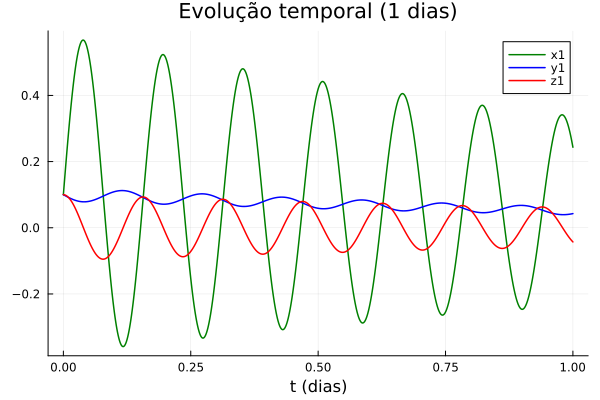
\includegraphics[width=0.6\textwidth]{00_TCC/01_LATEX/figuras/ch01_lorenz_80/evolucao_temporal_01.png}
	\caption{Simulação do modelo PE (1 dia).\label{fig:lorenz80_pe_1}}
\end{figure}

\chapter{Mori-Zwanzig}

\section{Introdução}
O principal objetivo do artigo de \citet{Chekroun2021} é simplificar o modelo de Lorenz 80, preservando seu comportamento. Para isso, utilizaremos o método de Mori-Zwanzig, que é uma abordagem física-estatística aplicável em sistemas como o L80.

O método de Mori-Zwanzig, desenvolvido por Robert Walter Zwanzig e Hajime Mori na segunda metade do século XX, é utilizado em sistemas hamiltonianos. Esse método consiste em classificar as variáveis do sistema em duas categorias: ``resolvidas'' e ``não resolvidas''. As variáveis resolvidas são aquelas cujos comportamentos e valores são bem conhecidos, enquanto as não resolvidas são aquelas para as quais não se possui informações diretas. Para substituir essas variáveis não resolvidas, o método introduz termos estocásticos, denominados ruídos (\textit{noise}), além de um termo de amortecimento (\textit{damping}), também conhecido como termo de memória (\textit{memory term}). Essa abordagem permite que o comportamento do sistema de interesse seja preservado de maneira adequada, mesmo sem conhecer completamente as variáveis não resolvidas.

Dada a relevância deste método para o trabalho de \citet{Chekroun2021}, optamos por incluir uma introdução ao formalismo de Mori-Zwanzig, a fim de proporcionar uma melhor compreensão de sua aplicação no contexto do modelo de Lorenz 80 e permitir uma base teórica sólida para eventuais explorações.

\section{Motivação}
Consideremos o exemplo de \citet[p.173]{Chorin2013}: um sistema com duas partículas em uma dimensão espacial, com Hamiltoniano dado por:
\begin{equation*}
	H = \frac{1}{2}(q_1^2 + q_2^2 + q_1^2 q_2^2 + p_1^2 + p_2^2)
\end{equation*}
onde $q_i$ e $p_i$, $i = 1, 2$, representam posições e momentos. Os osciladores harmônicos, uma vez em movimento, oscilam indefinidamente. As equações de movimento são expressas por:
\begin{align}
	\dot{q}_1 & = p_1, \nonumber             \\
	\dot{p}_1 & = -q_1(1 + q_2^2), \nonumber \\
	\dot{q}_2 & = p_2, \nonumber             \\
	\dot{p}_2 & = -q_2(1 + q_1^2).           
	\label{eq:exemplo-sistema-harmonico}
\end{align}

Suponha que os valores iniciais $q_1(0)$ e $p_1(0)$ sejam conhecidos. Assuma que $q_2(0)$ e $p_2(0)$ são amostrados a partir da função densidade de probabilidade:
\begin{equation*}
	W = \frac{e^{-H(q,p)}}{Z}   
\end{equation*}

Essa amostragem pode ser realizada, por exemplo, por meio do método de Monte Carlo via cadeia de Markov.

Dada uma amostra de $q_2(0)$ e $p_2(0)$, o sistema \eqref{eq:exemplo-sistema-harmonico} pode ser resolvido. Contudo, para cada nova amostra de $q_2(0)$ e $p_2(0)$, obtém-se uma trajetória distinta para $q_1(t)$ e $p_1(t)$. Em particular, pode-se querer calcular os valores esperados de $q_1$ e $p_1$ no tempo $t$, dados seus valores iniciais, os quais representam as melhores estimativas de $q_1(t)$ e $p_1(t)$:
\begin{equation*}
	\mathbb{E}[q_1(t)\mid q_1(0), p_1(0)], \quad \mathbb{E}[p_1(t)\mid q_1(0), p_1(0)].
\end{equation*}

Uma vez que $q_2$ e $p_2$ foram amostrados, o sistema completo de quatro equações pode ser resolvido. Isso pode ser feito repetidamente, permitindo calcular a média dos valores de $q_1(t)$ e $p_1(t)$ ao longo de várias execuções.

No entanto, há uma limitação: essa abordagem é adequada apenas para os instantes iniciais do sistema. À medida que o tempo avança, o valor esperado de $q_1(t)$ se distancia do valor real, comprometendo a precisão da aproximação.



\section{Prolegômenos}
\subsection{Escrevendo sistemas de EDO não lineares como sistemas de EDPs lineares}

Considere o sistema de equações diferenciais ordinárias (EDO) dado por:
\begin{equation}
	\frac{d}{dt} \phi(x,t) = R(\phi(x,t)), \quad \phi(x, 0) = x,
	\label{eq:sistema-edo}
\end{equation}

onde $R$ é uma função não linear, $\phi$ é uma função dependente do tempo, e $R$, $\phi$ e $x$ podem assumir dimensões infinitas, sendo formados pelos vetores $R_i$, $\phi_i$ e $x_i$, respectivamente.

A partir disso, podemos definir o \textit{Operador de Liouville} associado à equação \eqref{eq:sistema-edo} como:
\begin{equation}
	L = \sum_i R_i(x) \frac{\partial}{\partial x_i}
	\label{eq:liouville-operator}
\end{equation}

Utilizando o \textit{Operador de Liouville}, podemos transformar o sistema de EDOs não lineares em um sistema de equações diferenciais parciais (EDPs) lineares da forma:
\begin{equation}
	u_t = Lu, \quad u(x,0) = g(x)
	\label{eq:sistema-edp-linear}
\end{equation}

A solução desse sistema existe, é única, e é dada por:
\begin{equation}
	u(x,t) = g(\phi(x,t))   
	\label{eq:solucao-sistema-edp-linear}
\end{equation}
Portanto, temos que a equação \eqref{eq:sistema-edp-linear} é bem definida\footnote{Detalhes da demonstração podem ser encontrados em \citet[p.~181-182]{Chorin2013}}.

\subsection{Notação de semigrupo}
\subsection{Definição de semigrupo}
Tomemos $X$ um conjunto não vazio, dotado de uma operação binária $ * $, ou seja, $ X \times X \to X $, que satisfaz a propriedade de associatividade:
\begin{equation*}
	(a * b) * c = a * (b * c), \quad \forall a,b,c \in X.
\end{equation*}

\subsubsection{Introdução à notação}
A notação de semigrupo oferece uma forma compacta e eficiente de representar soluções para equações diferenciais, particularmente as parciais ou de evolução.

Considere o operador $\Delta$ definido por:
\begin{equation*}
	\Delta \psi = \psi_{xx}, \quad \text{onde $\psi$ é uma função suave}.
\end{equation*}
Agora, considere a equação diferencial:
\begin{equation*}
	\frac{dv}{dt} - kv = 0, \quad v(0) = v_0,
\end{equation*}
cuja solução é bem conhecida: $ v(t) = v_0 e^{kt} $.

De forma análoga, considere a equação do calor:
\begin{equation*}
	v_t - \frac{1}{2} \Delta v = 0, \quad v(x, 0) = \phi(x),
\end{equation*}
onde $v_t$ é a derivada de $v$ em relação ao tempo e $\phi(x)$ é a condição inicial. Em vez de resolver diretamente, expressamos a solução utilizando a notação de semigrupo:
\begin{equation*}
	v(t) = e^{\frac{1}{2}t \Delta} \phi.
\end{equation*}
Aqui, $\mathbb{E}^{\frac{1}{2}t \Delta}$ é um operador semigrupo gerado pela operação de difusão (pelo operador $\Delta$). Ele é aplicado à condição inicial $\phi(x)$, e a solução $v(t)$ descreve a evolução temporal de $v(x,t)$ ao longo do tempo $t$. Essa notação permite representar soluções de equações diferenciais de maneira compacta, explorando a estrutura associativa da operação de semigrupo. Especificamente, ela satisfaz a propriedade de composição:
\begin{equation*}
	e^{\frac{1}{2}(t+s)\Delta} = e^{\frac{1}{2}t \Delta} e^{\frac{1}{2}s \Delta}.
\end{equation*}

\subsection{Aplicação da notação}
Dada a notação de semigrupo apresentada anteriormente, aplicamos esta notação à equação \eqref{eq:solucao-sistema-edp-linear}:
\begin{equation}
	e^{tL}g(x) = g(\phi(x,t))
	\label{eq:solucao-sistema-edp-linear-semigrupo}
\end{equation}

Note que $\mathbb{E}^{tL}x$ não representa uma avaliação direta de $\mathbb{E}^{tL}$, mas sim a ação do operador $\mathbb{E}^{tL}$ sobre o vetor formado pelos componentes $x_i$. Além disso, a função $g$ comuta com a variação temporal das condições iniciais de $x_i$. 

Vale destacar que $g$ é uma função independente do tempo em relação às variáveis que descrevem o sistema físico, e sua variação ocorre exclusivamente devido à mudança dessas variáveis ao longo do tempo. Assim, a equação \eqref{eq:sistema-edp-linear} pode ser expressa como:
\begin{equation}
	Le^{tL} = e^{tL}L
\end{equation}

Essa mesma relação se aplica a matrizes: sejam $A$ e $B$ duas matrizes, então a seguinte identidade é válida:
\begin{equation}
	\exp(t(A+B)) = \exp(tA) + \int_0^t \exp\left((t-s)(A+B)\right)B\exp(sA) \, ds
	\label{eq:formula-de-duhamel}
\end{equation}

Esta equação, conhecida como \textit{Fórmula de Duhamel} ou \textit{fórmula de Dyson}, é bem definida.

\subsection{Polinômios Hermitianos}

Primeiramente, definimos o produto interno como:
\begin{equation}
	\langle u, v \rangle = \int_{-\infty}^{+\infty} \frac{e^{-x^2/2}}{\sqrt{2 \pi}} u(x) v(x) \, dx
	\label{eq:produto-interno-hermitiano-unidimensional}
\end{equation}

Os polinômios $p_n(x)$ e $p_m(x)$ são ortonormais em relação a esse produto interno \eqref{eq:produto-interno-hermitiano-unidimensional} quando satisfazem a seguinte condição:
\begin{equation*}
	\langle p_n, p_m \rangle = \int_{-\infty}^{\infty} e^{-x^2/2} p_n(x) p_m(x) \, dx = \delta_{nm},
\end{equation*}
em que $\delta_{nm}$ é o delta de Kronecker, que apresenta as propriedades:

\begin{enumerate}
	\item \textbf{Ortogonalidade}: Para $n \neq m$, os polinômios são ortogonais, ou seja, o produto interno entre eles é nulo:
	      \begin{equation*}
	      	\langle p_n, p_m \rangle = 0 \quad \text{quando} \quad n \neq m
	      \end{equation*}
	      	          
	\item \textbf{Normalização}: Para $n = m$, os polinômios são normalizados, de modo que o produto interno é igual a 1:
	      \begin{equation*}
	      	\langle p_n, p_n \rangle = 1
	      \end{equation*}
\end{enumerate}

No caso $n$-dimensional, o produto interno se generaliza para:
\begin{equation*}
	\langle u, v \rangle = \int_{-\infty}^{+\infty} \cdots \int_{-\infty}^{+\infty} (2 \pi)^{-n/2} \exp \left(-\sum_{i=1}^n \frac{x_i^2}{2} \right) u(x) v(x) \, dx_1 \ldots dx_n
\end{equation*}

De forma mais geral, se $H(q, p)$ é um Hamiltoniano, é possível definir uma família de polinômios nas variáveis $q$ e $p$ que sejam ortonormais com respeito à densidade canônica $Z^{-1} e^{-H/T}$. Os polinômios que satisfazem essa condição ainda são chamados de \textit{polinômios hermitianos}.

Por fim, para o formalismo de Mori-Zwanzig, consideraremos um espaço $n$-dimensional $\Gamma$ com uma densidade de probabilidade dada. Dividiremos as coordenadas em dois tipos: $\hat{x}$ e $\tilde{x}$. Seja $g$ uma função de $x$; então $\mathbb{P}g = \mathbb{E}[g \mid \hat{x}]$ é uma projeção ortogonal sobre o subespaço das funções de $\hat{x}$.Temos que essa projeção gera um subespaço de polinômios hermitianos que são funções de $\hat{x}$ e projetando sobre esses polinômios.


\section{Mori-Zwanzig}
\subsection{Construção}
Tomemos novamente o sistema \eqref{eq:sistema-edo}, reproduzido abaixo:
\begin{equation*}
	\frac{d}{dt} \phi(x,t) = R(\phi(x,t)), \quad \phi(x, 0) = x,
\end{equation*}

Lembremos que a equação é composta por componentes de dimensão $n$. Dentre essas $n$ componentes, definimos as primeiras $m$ componentes de $\phi$, com $m < n$, como as variáveis de interesse. Em seguida, classificamos $\hat{\phi}$ como as variáveis ``resolvidas'' e $\tilde{\phi}$ como as variáveis ``não resolvidas'':
\begin{equation*}
	\phi = (\hat{\phi}, \tilde{\phi}), \quad \hat{\phi} = \left(\phi_1, \ldots, \phi_m \right), \quad \tilde{\phi} = \left(\phi_{m+1}, \ldots, \phi_n\right)
\end{equation*}
O mesmo vale para $x$ e $R$: $x = (\hat{x}, \tilde{x})$ e $R = (\hat{R}, \tilde{R})$. A partir das variáveis resolvidas, buscamos criar predições para o modelo de interesse, utilizando as soluções de uma parte da equação.

Com base no \textit{Operador de Liouville} e na \textit{notação de semigrupo}, podemos reescrever as componentes de $\hat{\phi}$ como\footnote{Note que cada componente depende de \textbf{todos} os valores de $x$. Portanto, se $\tilde{x}$ for aleatório, então $\hat{\phi}$ também será.}:
\begin{equation*}
	\hat{\phi}_j(x,t) = e^{tL}x_j, \quad 1 \leq j \leq m
\end{equation*}
Ainda na notação de semigrupo, a equação dessas componentes é dada por:
\begin{equation}
	\frac{\partial}{\partial t}e^{tL}x_j = Le^{tL}x_j = e^{tL}Lx
	\label{eq:mori-zwanzig-notacao-semigrupo}
\end{equation}

A partir da \textit{projeção ortogonal} introduzida na seção anterior, definimos $\mathbb{P}$ como a projeção dada por: $\mathbb{P}g(x) = \mathbb{E}[g|\hat{x}]$. Assumimos que, no instante $t = 0$, conhecemos a densidade conjunta de todas as variáveis $x$, mas apenas os dados iniciais $\hat{x}$ são conhecidos. A densidade das variáveis em $\tilde{x}$ é, então, a densidade conjunta de todas as variáveis $x$ com $\hat{x}$ fixado. Assim, $\mathbb{P}$ é uma projeção sobre um espaço de funções com variáveis fixas e, portanto, independente do tempo.

As projeções $\mathbb{P}\hat{\phi}(t) = \mathbb{E}[\hat{\phi}(t) | \hat{x}]$ são de nosso maior interesse, pois estimam o comportamento do sistema a partir de um conjunto reduzido de variáveis.

Definindo $\mathbb{Q} = I - \mathbb{P}$ e considerando que as seguintes propriedades são válidas para quaisquer projeções ortogonais:
\begin{enumerate}
	\item $\mathbb{P}^2 = \mathbb{P}$;
	\item $\mathbb{Q}^2 = \mathbb{Q}$;
	\item $\mathbb{P}\mathbb{Q} = 0$.
\end{enumerate}

Podemos reescrever a equação \eqref{eq:mori-zwanzig-notacao-semigrupo} como:
\begin{equation}
	\frac{\partial }{\partial t}e^{tL}x_j = e^{tL}\mathbb{P}Lx_j + e^{tL}\mathbb{Q}Lx_j
	\label{eq:mori-zwanzig-pre-mz}
\end{equation}

Utilizando agora a \textit{fórmula de Dyson}, com $A = \mathbb{Q}L$ e $B = \mathbb{Q}L$, obtemos:
\begin{equation}
	e^{tL} = e^{t\mathbb{Q}L} + \int_0^t e^{(t-s)L} \mathbb{P}L e^{s\mathbb{Q}L} \, ds
	\label{eq:mori-zwanzig-dyson-mz}
\end{equation}

Pela linearidade da equação de Liouville e a partir das equações \eqref{eq:mori-zwanzig-pre-mz} e \eqref{eq:mori-zwanzig-dyson-mz}, obtemos:
\begin{equation}
	\frac{\partial}{\partial t} e^{tL} x_j = e^{tL} \mathbb{P}L x_j + e^{t\mathbb{Q}L} \mathbb{Q}L x_j + \int_0^t e^{(t-s)L} \mathbb{P}L e^{s\mathbb{Q}L} \mathbb{Q}L x_j \, ds
	\label{eq:mori-zwanzig}
\end{equation}

A equação acima expressa a \textit{equação de Mori-Zwanzig}.

\subsection{Análise termo a termo}
\subsubsection{Primeiro termo}
O primeiro termo é dado por:  
\begin{equation}
	e^{tL} \mathbb{P}L x_j
	\label{eq:primeiro-termo-mz}
\end{equation}

Observe que:  
\begin{equation*}
	Lx_j = \sum_i R_i\left(\frac{\partial}{\partial x_i}\right)x_j = R_j(x)
\end{equation*}

Portanto,  
\begin{equation*}
	\mathbb{P}Lx_j = \mathbb{E}[R_j(x)\,|\,\hat{x}] \quad \text{Note que esta é uma função exclusivamente de $\hat{x}$.}
\end{equation*}

Com isso, podemos concluir que:  
\begin{equation*}
	e^{tL}\mathbb{P}Lx_j = \bar{R}_j\left(\hat{\phi}(x,t)\right)
\end{equation*}

Mais do que isso: o primeiro termo representa a dinâmica própria do sistema nas variáveis resolvidas. Além disso, trata-se de um termo markoviano, pois depende apenas do estado atual do sistema no tempo $t$.

\subsubsection{Segundo termo}
Para o segundo termo, definimos:
\begin{equation*}
	w_j = e^{t\mathbb{Q}L} \mathbb{Q}L x_j
\end{equation*}

Por definição, temos:
\begin{align}
	\frac{\partial}{\partial t} w_j(x,t) & = \mathbb{Q}L w_j(x,t),\\
	w_j(x,0)                             & = \mathbb{Q}L x_j = (I - \mathbb{P})R_j(x) = R_j(x) - \mathbb{E}[R_j \mid \hat{x}]. 
    \label{eq:mori-zwanzig-dinamica-ortogonal}
\end{align}

Note que $w_j(x,0) = \mathbb{Q}Lx_j = R_j(x) - \mathbb{E}[R_j(x) \mid \hat{x}]$ representa a \textit{parte flutuante} da variável $R_j(x)$, ou seja, o componente imprevisível dado $\hat{x}$. Essa parte evolui de acordo com as \textit{dinâmicas ortogonais}, de modo que $\mathbb{P} w_j(x,t) = 0$ para todo $t$, mantendo o termo como um ruído puramente não resolvido ao longo do tempo.

Mais especificamente, o subespaço do ruído (\textit{noise subspace}) é formado pelas componentes das funções que são ortogonais às funções de $\hat{x}$, geralmente, isso corresponde a termos que dependem de $\tilde{x}$. 

\subsubsection{Terceiro termo}
O terceiro termo, dado por:
\begin{equation*}
	\int_0^t e^{(t-s)L} \mathbb{P}L e^{s\mathbb{Q}L} \mathbb{Q}L x_j
\end{equation*}
é classificado como o termo de memória  (\textit{memory term}), já que este envolve a integração de quantidades que dependem de estados anteriores ao atual.

Tomemos que $\mathbb{P}$ seja projete na extensão dos polinômios hermitianos $H-1, H_2, \ldots$ com argumentos em $\hat{x}$. Assim, para dada função $\psi$, temos que: $\mathbb{P}\psi = \sum (\psi, H_k)H_k$, assim, temos:
\begin{align*}
	\mathbb{P}Le^{s\mathbb{Q}L} \mathbb{Q}Lx_j & = \mathbb{P}L(\mathbb{P} + \mathbb{Q})e^{s\mathbb{Q}L} \mathbb{Q}Lx_j                           \\
	                                           & = \mathbb{P}L\mathbb{Q}e^{s\mathbb{Q}L} \mathbb{Q}Lx_j                                          \\
	                                           & = \sum_k \langle L\mathbb{Q}e^{s\mathbb{Q}L} \mathbb{Q}Lx_j, H_k(\hat{x}) \rangle H_k(\hat{x}). 
\end{align*}

O produto interno é definido como um valor esperado com respeito à densidade de probabilidade inicial. Vamos assumir que $L$ é antissimétrico, ou seja, $(u, Lv) = -(Lu, v)$, então:
\begin{align*}
	(L Q e^{s Q L} Q L x_j, H_k(\hat{x})) 
	  & = - (Q e^{s Q L} Q L x_j, L H_k)  \\
	  & = - (e^{s Q L} Q L x_j, Q L H_k). 
\end{align*}

Tanto $Q L x_j$ quanto $Q L H_k$ estão no subespaço de ruído, e $\mathbb{E}^{s Q L} Q L x_j$ é uma solução no tempo $s$ da equação de dinâmica ortogonal com dados no subespaço de ruído; $P L e^{s Q L} Q L x_j$ é então uma \textbf{soma de covariâncias temporais de ruídos}.



\section{Voltando à motivação}

\subsection{Introdução}
Inicialmente, vamos relembrar o problema em questão: temos um sistema hamiltoniano, com o hamiltoniano definido por  
\begin{equation*}
	H = \frac{1}{2}(q_1^2 + q_2^2 + q_1^2 q_2^2 + p_1^2 + p_2^2).
\end{equation*}

As equações do movimento associadas são dadas por:  
\begin{align*}
	\dot{q}_1 & = p_1, \nonumber             \\
	\dot{p}_1 & = -q_1(1 + q_2^2), \nonumber \\
	\dot{q}_2 & = p_2, \nonumber             \\
	\dot{p}_2 & = -q_2(1 + q_1^2).           
\end{align*}

Aplicando o \textit{Operador de Liouville}, obtemos:  
\begin{equation*}
	L = p_1 \frac{\partial}{\partial q_1} - q_1(1 + q_2^2)\frac{\partial}{\partial p_1}
	+ p_2 \frac{\partial}{\partial q_2} - q_2(1 + q_1^2)\frac{\partial}{\partial p_2}.
\end{equation*}

Como antes, assumimos que os valores iniciais $q_1(0)$ e $p_1(0)$ são conhecidos, enquanto $q_2$ e $p_2$ são definidos por uma função densidade de probabilidade dada por:
\begin{equation*}
	W(x) = \exp\left(\frac{-H(q_1,p_1,q_2,p_2)}{Z}\right) \quad \text{(uma densidade canônica com temperatura $T = 1$).}
\end{equation*}

Nosso objetivo é avaliar $q_1(t)$ e $p_1(t)$ a partir das equações de Mori-Zwanzig \eqref{eq:mori-zwanzig}.

\subsection{Primeira aproximação}
Dada a natureza do sistema, é necessário realizar uma aproximação para introduzir o termo de memória. Sabemos que as dinâmicas ortogonais descritas em \eqref{eq:mori-zwanzig-dinamica-ortogonal} são aproximadamente equivalentes às dinâmicas completas, uma vez que não são sensíveis às variáveis resolvidas. Com base nisso, a aproximação consiste em substituir $e^{t\mathbb{Q}L}$ por $e^{tL}$ no termo de memória. Essa substituição é válida quando a influência das variáveis resolvidas sobre as não resolvidas é pequena\footnote{Essa substituição é justificada quando o acoplamento entre as variáveis resolvidas e não resolvidas é fraco.}. 

Dito isso, podemos iniciar a manipulação algébrica. Um operador comuta com qualquer função de si mesmo, de modo que:
\begin{equation*}
	\mathbb{Q}Le^{s\mathbb{Q}L} = e^{s\mathbb{Q}L} \mathbb{Q}L.
\end{equation*}
Usando essa identidade e substituindo $e^{s\mathbb{Q}L} \to e^{sL}$ no lado direito da igualdade, obtemos:
\begin{equation*}
	\mathbb{P}Le^{s\mathbb{Q}L} \approx Le^{sL} - e^{sL} \mathbb{Q}L.
\end{equation*}
Então,
\begin{equation*}
	e^{(t-s)L} \mathbb{P}Le^{s\mathbb{Q}L} \approx e^{(t-s)L} Le^{sL} - e^{(t-s)L} e^{sL} \mathbb{Q}L = e^{tL} \mathbb{P}L,
\end{equation*}
o que torna o integrando no termo integral da equação de Mori-Zwanzig independente de $s$, resultando em:
\begin{equation*}
	\int_0^t e^{tL} \mathbb{P}L \mathbb{Q}L x_j \, ds = t e^{tL} \mathbb{P}L \mathbb{Q}L x_j,
\end{equation*}
onde $\hat{x}$ é o vetor com componentes $x_1 = q_1$ e $x_2 = p_1$. O termo de memória foi assim reduzido a um operador diferencial multiplicado pelo tempo $t$. Note que $t = 0$ corresponde ao instante em que os valores iniciais de $q_1(t)$ e $p_1(t)$ são atribuídos, ou seja, quando não há incerteza. Essa aproximação também pode ser justificada assumindo que o integrando no termo de memória é aproximadamente constante em $s$, e portanto pode ser avaliado em $s = 0$.

As equações com o termo integral simplificado constituem o chamado modelo-$t$. Reunindo os termos, temos:
\begin{equation*}
	\frac{d}{dt} e^{tL} \hat{x} = e^{tL} \mathbb{P}L \hat{x} + t e^{tL} \mathbb{P}L \mathbb{Q}L \hat{x} + e^{tL} \mathbb{Q}L \mathbb{Q}L x_j.
\end{equation*}

No caso particular considerado, com os componentes $x_j = q_1$ e $x_j = p_1$, obtemos:
\begin{align*}
	Lq_1                        & = p_1, \\
	\mathbb{P}Lq_1              & = p_1, \\
	\mathbb{Q}Lq_1              & = 0,   \\
	L\mathbb{Q}Lq_1             & = 0,   \\
	\mathbb{P}L \mathbb{Q}L q_1 & = 0,   
\end{align*}
e
\begin{align*}
	Lp_1 &= -q_1(1 + q_2^2),\\
	\mathbb{P}Lp_1 &= -q_1\left(1 + \frac{1}{1 + q_1^2}\right),\\
	\mathbb{Q}Lp_1 &= -q_1(1 + q_2^2) + q_1\left(1 + \frac{1}{1 + q_1^2}\right),\\
	L\mathbb{Q}Lp_1 &= p_1\left(- (1 + q_2^2) + \left(1 + \frac{1}{1 + q_1^2} \right) \right) - \frac{2q_1^2}{(1 + q_1^2)^2} - 2q_1 q_2 p_2, \\
	\mathbb{P}L\mathbb{Q}Lp_1 & = -\frac{2q_1^2 p_1}{(1 + q_1^2)^2}.
\end{align*}

Assim, as equações aproximadas de movimento para $q_1$ e $p_1$ tornam-se:
\begin{align}
	\frac{d}{dt} q_1 & = p_1, \nonumber \\
	\frac{d}{dt} p_1 & = -q_1\left(1 + \frac{1}{1 + q_1^2}\right) - 2t\frac{q_1^2 p_1}{(1 + q_1^2)^2} + e^{tL} \mathbb{Q}L \mathbb{Q}L p_1. \label{eq:mori-zwanzig-sistema-hamiltoniano}
\end{align}

Suponha agora que desejamos conhecer apenas as quantidades:
\begin{equation*}
	\mathbb{E}[q_1(t) \mid q_1(0), p_1(0)], \quad \mathbb{E}[p_1(t) \mid q_1(0), p_1(0)],
\end{equation*}
ou seja, as esperanças condicionais de $q_1(t)$ e $p_1(t)$ dado $q_1(0), p_1(0)$. 

Uma equação para essas quantidades pode ser obtida aplicando o operador $\mathbb{P}$ às equações \eqref{eq:mori-zwanzig-sistema-hamiltoniano}, lembrando que, por definição, $\mathbb{P}q_1(t) = \mathbb{E}[q_1(t) \mid q_1(0), p_1(0)]$, e de forma análoga para $p_1(t)$. Nesse processo, o termo de ruído desaparece.

Contudo, surge um problema: a média de uma função de uma variável, em geral, não é igual à função da média. Para contornar essa dificuldade, uma simplificação adicional é necessária. Essa complicação pode ser evitada ao considerar trajetórias específicas das variáveis resolvidas, onde tal distinção se torna irrelevante, permitindo aplicar diretamente as equações aproximadas sem as dificuldades associadas às dinâmicas ortogonais.

\subsection{Segunda aproximação}

Assuma que, para as funções no lado direito das equações \eqref{eq:mori-zwanzig-sistema-hamiltoniano}, a operação de média e a avaliação da função comutam. Isso significa que, por exemplo,
\begin{equation*}
    \mathbb{E}[(1 + q_1^2(t))^{-1} \mid q_1(0), p_1(0)] \approx \left(1 + \mathbb{E}[q_1(t) \mid \cdot]^2\right)^{-1}.
\end{equation*}

Essa aproximação de campo médio é válida quando o ruído é suficientemente pequeno. No caso limite em que o ruído é nulo, a aproximação torna-se exata. No problema específico considerado, essa hipótese deve ser razoável caso os dados iniciais sejam amostrados de uma densidade canônica com temperatura baixa. Aqui, utilizamos uma temperatura inicial \(T = 1\).

Com isso, definimos:
\begin{equation*}
    Q_1(t) = \mathbb{E}[q_1(t) \mid q_1(0), p_1(0)], \quad P_1(t) = \mathbb{E}[p_1(t) \mid q_1(0), p_1(0)].
\end{equation*}

As equações aproximadas de movimento passam a ser:
\begin{align*}
    \frac{d}{dt} Q_1 &= P_1,\\
    \frac{d}{dt} P_1 &= -Q_1\left(1 + \frac{1}{1 + Q_1^2} \right) - t \cdot \frac{2 Q_1^2 P_1}{(1 + Q_1^2)^2}.
\end{align*}

A equação acima é resolvível numericamente e, a partir dela, temos a aproximação de Mori-Zwanzig para o nosso problema de interesse.

%%%%%%%%%%%%%%%%%%%%%%%%%%%% APÊNDICES E ANEXOS %%%%%%%%%%%%%%%%%%%%%%%%%%%%%%%%

% Um apêndice é algum conteúdo adicional de sua autoria que faz parte e
% colabora com a ideia geral do texto mas que, por alguma razão, não precisa
% fazer parte da sequência do discurso; por exemplo, a demonstração de um
% teorema intermediário, as perguntas usadas em uma pesquisa qualitativa etc.
%
% Um anexo é um documento que não faz parte da tese (em geral, nem é de sua
% autoria) mas é relevante para o conteúdo; por exemplo, a especificação do
% padrão técnico ou a legislação que o trabalho discute, um artigo de jornal
% apresentando a percepção do público sobre o tema da tese etc.
%
% Os comandos appendix e annex reiniciam a numeração de capítulos e passam
% a numerá-los com letras. "annex" não faz parte de nenhuma classe padrão,
% foi criado para este modelo. Se o trabalho não tiver apêndices ou anexos,
% remova estas linhas.
%
% Diferentemente de \mainmatter, \backmatter etc., \appendix e \annex não
% forçam o início de uma nova página. Em geral isso não é importante, pois
% o comando seguinte costuma ser "\chapter", mas pode causar problemas com
% a formatação dos cabeçalhos. Assim, vamos forçar uma nova página antes
% de cada um deles.

%%%% Apêndices %%%%

\cleardoublepage

\pagestyle{appendix}

\appendix

% \addappheadtotoc acrescenta a palavra "Apêndice" ao sumário; se
% só há apêndices, sem anexos, provavelmente não é necessário.
\addappheadtotoc

%!TeX root=../tese.tex
%("dica" para o editor de texto: este arquivo é parte de um documento maior)
% para saber mais: https://tex.stackexchange.com/q/78101

\chapter{Perguntas frequentes sobre o modelo}

\begin{itemize}

\item \textbf{Não consigo decorar tantos comandos!}\\
Use a colinha que é distribuída juntamente com este modelo (\url{gitlab.com/ccsl-usp/modelo-latex/raw/main/pre-compilados/colinha.pdf?inline=false}).

\item \textbf{Estou tendo problemas com caracteres acentuados.}\\
Versões modernas de \LaTeX{} usam UTF-8, mas arquivos antigos podem usar outras codificações (como ISO-8859-1, também conhecido como latin1 ou Windows-1252). Nesses casos, use \textsf{\textbackslash{}usepackage[latin1]\{inputenc\}} no preâmbulo do documento. Você também pode representar os caracteres acentuados usando comandos \LaTeX{}: \textsf{\textbackslash\textquotesingle{}a} para á, \textsf{\textbackslash{}c\{c\}} para cedilha etc., independentemente da codificação usada no texto\footnote{Você pode consultar os comandos desse tipo mais comuns em \url{en.wikibooks.org/wiki/LaTeX/Special_Characters}. Observe que a dica sobre o pingo do i \emph{não} é mais válida atualmente; basta usar \textsf{\textbackslash\textquotesingle{}i}.}.

\item \textbf{É possível resumir o nome das seções/capítulos que aparece no topo das páginas e no sumário?}\\
Sim, usando a sintaxe \textsf{\textbackslash{}section[mini-titulo]\{titulo enorme\}}. Isso é especialmente útil nas legendas (\textit{captions}\index{Legendas}) das figuras e tabelas, que muitas vezes são demasiadamente longas para a lista de figuras/tabelas.

\item \textbf{Existe algum programa para gerenciar referências em formato bibtex?}\\
Sim, há vários. Uma opção bem comum é o JabRef; outra é usar Zotero\index{Zotero} ou Mendeley\index{Mendeley} e exportar os dados deles no formato .bib.

\item \textbf{Posso usar pacotes \LaTeX{} adicionais aos sugeridos?}\\
Com certeza! Você pode modificar os arquivos o quanto desejar, o modelo serve só como uma ajuda inicial para o seu trabalho.

\end{itemize}

\par

%%%% Anexos %%%%

\cleardoublepage

\pagestyle{appendix} % repete o anterior, caso você não use apêndices

\annex

% \addappheadtotoc acrescenta a palavra "Anexo" ao sumário; se
% só há anexos, sem apêndices, provavelmente não é necessário.
\addappheadtotoc

\par


%%%%%%%%%%%%%%% SEÇÕES FINAIS (BIBLIOGRAFIA E ÍNDICE REMISSIVO) %%%%%%%%%%%%%%%%

% O comando backmatter desabilita a numeração de capítulos.
\backmatter

\pagestyle{backmatter}

% Espaço adicional no sumário antes das referências / índice remissivo
\addtocontents{toc}{\vspace{2\baselineskip plus .5\baselineskip minus .5\baselineskip}}

% A bibliografia é obrigatória

\printbibliography[
  title=\refname\label{sec:bib}, % "Referências", recomendado pela ABNT
  %title=\bibname\label{sec:bib}, % "Bibliografia"
  heading=bibintoc, % Inclui a bibliografia no sumário
]

\printindex % imprime o índice remissivo no documento (opcional)

\end{document}
